\documentclass[11pt, a4paper]{article}
\usepackage[spanish]{babel}
\usepackage{amssymb}
\usepackage{graphicx}
\usepackage{amsmath}
\begin{document}
	\setcounter{section}{3}
	\newcommand\Tau{\mathrm{T}}
\section{Un Resultado Importante de Semejanzas Espirales}
\setcounter{footnote}{1}
Una semejanza espiral\footnote{Si quieres impresionar a tus amigos con tu vocabulario matem\'atico, una semejanza espiral a veces se llama $similitud$ y una dilataci\'on a veces se llama $homotecia$. (En realidad, no son exactamente la misma cosa, pero shhh!)} sobre un punto $O$ (Conocido como el centro de una semejanza espiral) es una composici\'on de una rotaci\'on y una dilataci\'on, ambos centrados en $O$.
\setcounter{figure}{3}
\begin{figure}[h]
	\centering
	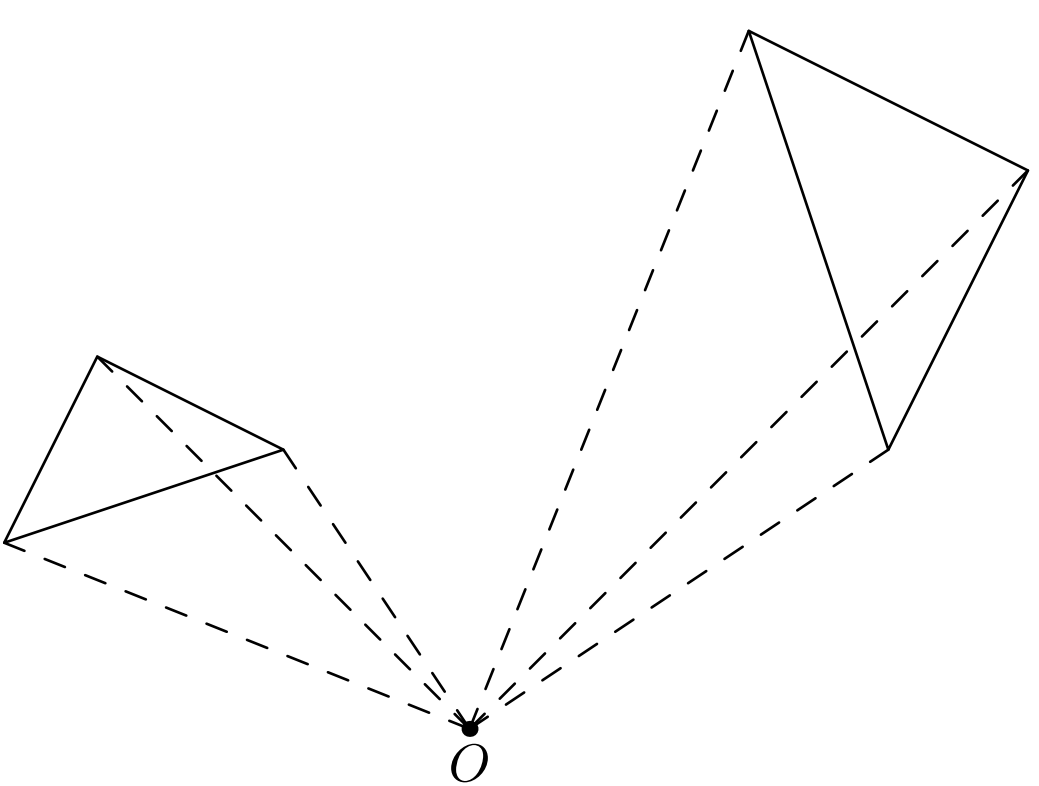
\includegraphics[scale=0.3]{p4.1}
	\caption{Ejemplo de semejanza espiral}
\end{figure}


Por ejemplo, en el plano complejo, si $O=0$, entonces semejanzas espirales son descritas por la multiplicaci\'on de un n\'umero complejo distinto a cero. Esto es, que las espirales semejantes tienen la forma $z \mapsto \alpha z$, donde $\alpha \ \in \mathbb{C} \setminus \{0\}$ Aqu\'i $|\alpha|$ es el factor de dilataci\'on, y arg $\alpha$ es el \'angulo de rotaci\'on. Es f\'acil deducir de aqu\'i que si el centro de la semejanza espiral es otro punto, digamos $z_0$, entonces la transformaci\'on es dada por $z \mapsto z_0 + \alpha (z - z_0)$ (¿Por qué?)
\\
\textbf{Hecho 4.} Sean $A, B, C, D$ cuatro puntos distintos en el plano, tal que $ABCD$ no es un paralelogramo. Entonces existe una \'unica semejanza espiral que env\'ia $A$ a $B$, y $C$ a $D$.\\


$Prueba$. Sean $a,b,c,d$ los n\'umeros complejos correspondientes a los puntos $A,B,C,D$. Sabemos que una semjanza espiral tiene la forma de $\Tau (z) = z_0 + \alpha(z + z_0) $, donde $z_0$ es el centro de la semejanza espiral, y $\alpha$ es informaci\'on acerca de la rotaci\'on y dilataci\'on. As\'i que nos gustar\'ia encontrar $\alpha$ y $z_0$ tal que $\Tau (a) = c$ y $\Tau (b) = d$. Esto llevar\'ia a resolver el sistema \\


\hfil $z_0 + \alpha (a - z_0) = c$, \hfil  $z_0 + \alpha (b - z_0) = d$
\newpage
Resolviendo, vemos que la \'unica soluci\'on es \\\\
\hfil $\alpha = \frac{c-d}{a-b}$, \hfil $z_0 = \frac{ad - bc}{a-b-c+d}$
Como $ABCD$ no es un paralelogramo, vemos que $a-b-c+d \ne 0$, as\'i que est\'a es la \'unica soluci\'on al sistema. Por lo tanto existe una \'unica semejanza espiral que envi\'ia $A$ a $B$ y $C$ a $D$. \hfill $\square$ \\

\textbf{Ejercicio 4.}¿C\'omo podemos determinar r\'apidamente el valor $\alpha$ en la prueba de arriba sin siquiera necesitar escribir el sistema de ecuaciones?\\

\textbf{Ejercicio 5.} Da un argumento geom\'etrico de por qu\'e la semejanza espiral, si existe, debe ser \'unica. (Pista: Sup\'on que $\Tau_1$ y $\Tau_2$ son dos de las tales semejanzas espirales, entonces  ¿Qu\'e podemos decir de $\Tau_1 \circ \Tau_2^{-1}$\\

Ahora llegamos al resultado clave de esta secci\'on. Nos da una muy simple y \'util descripci\'on del centro de una semejanza espiral. Puede ser muy \'util encontrar semejanzas espirales muy sutiles escondidas en un problema de geometr\'ia. Recuerda esto!
\\

\textbf{(Muy \'util) Hecho 5.} Sean $A, B, C, D$ cuatro puntos distintos en el plano, tal que $AC$ no es paralelo a $BD$. Las l\'ineas $AC$ y $BD$ se encuentran en $X$. Sea $O$ el punto de intersecci\'on distinto a $X$ de los circunc\'irculos de $ABX$ y $CDX$. Entonces $O$ es el centro de una \'unica semejanza espiral que env\'ia $A$ a $C$ y $B$ a $D$.
\setcounter{figure}{4}
\begin{figure}[h]
	\centering
	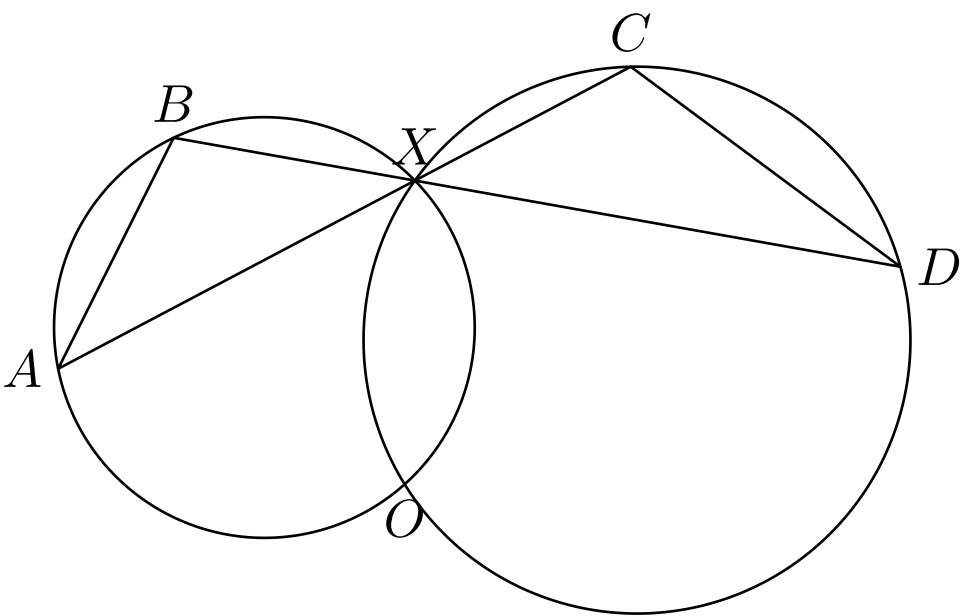
\includegraphics[scale=0.4]{p4.2}
	\caption{Diagrama del Hecho 5.}
\end{figure}

$Prueba.$ Damos una prueba solo para la configuraci\'on que est\'a arriba. Como $ABXO$ y $CDOX$ son c\'iclicos, tenemos que $\angle OBD = \angle OAC$ y $\angle OCA = \angle ODB$. Luego sigue que los tri\'angulos $AOC$ y $BOD$ son semejantes. Por lo tanto, la semejanza espiral con centro en $O$ que env\'ia $A$ a $C$ tambi\'en debe env\'iar $B$ a $D$.\\

\textbf{Ejercicio 6.} Reescribe la prueba de arriba usando \'angulos dirigidos m\'odulo $\pi$ tal que que funcione para todas las configuraciones. \\

Finalmente, vale la pena mencionar que las semejanzas espirales frecuentemente vienen en pares. Si podemos env\'iar $AB$ a $CD$, entonces tambi\'en facilmente podemos env\'iar $AC$ a $BD$.
\\

\textbf{Hecho 6.} Si $O$ es el centro de una semejanza espiral que env\'ia $A$ a $C$ y $B$ a $D$, entonces $O$ es tambi\'en centro de la semejanza espiral que env\'ia $A$ a $B$ y $C$ a $D$.\\

$Prueba.$ Como la semejanza espiral mantiene los mismo \'angulos en $O$, tenemos $\angle AOB = \angle COD$. Tambi\'en la raz\'on de la dilataci\'on de la primera semejanza espiral es $OC/OA = OD/OB.$ As\'i que la rotaci\'on con un \'angulo $\angle AOB = \angle COD$ y la dilataci\'on con raz\'on $OB/OA = OD/OC$ env\'ia $A$ a $B$, y $C$ a $D$, como quer\'iamos. \hfill $\square$


\textbf{Ejercicio 7.} Dedude el Hecho 6 utilizando el Hecho 2 y 5. \\

Ahora, aplicaremos estos resultados para nuestra configuraci\'on de la secci\'on 2.
\\

\textbf{Hecho 7.} Sea M el punto de Miquel del cuadril\'ater $ABCD$. Luego $M$ es el centro de la semejanza espiral que env\'ia a $AB$ a $CD$, como tambi\'en el centro de la semejanza espiral que env\'ia a $AD$ a $BC$ \\

\textbf{Ejercicio 8} Probar el Hecho 7. \\

Vamos a enfocarnos en cuadril\'ateros c\'iclicos y continuar la configuraci\'on del Hecho 3. \\

\textbf{Hecho 8.} Sea $ABCD$ un cuadril\'atero c\'iclico con circuncentro $O$. Las l\'ineas $AB$ y $CD$ se chocan en en $Q$, y las l\'ineas $DA$ y $CB$ se chocan en $R$. Sea $M$ el punto de Miquel de $ABCD$ (Que est\'a en la l\'inea QR, por el Hecho 3). Entonces $OM$ es perpendicular a $QR$.
\newpage
\begin{figure}[h]
	\centering
	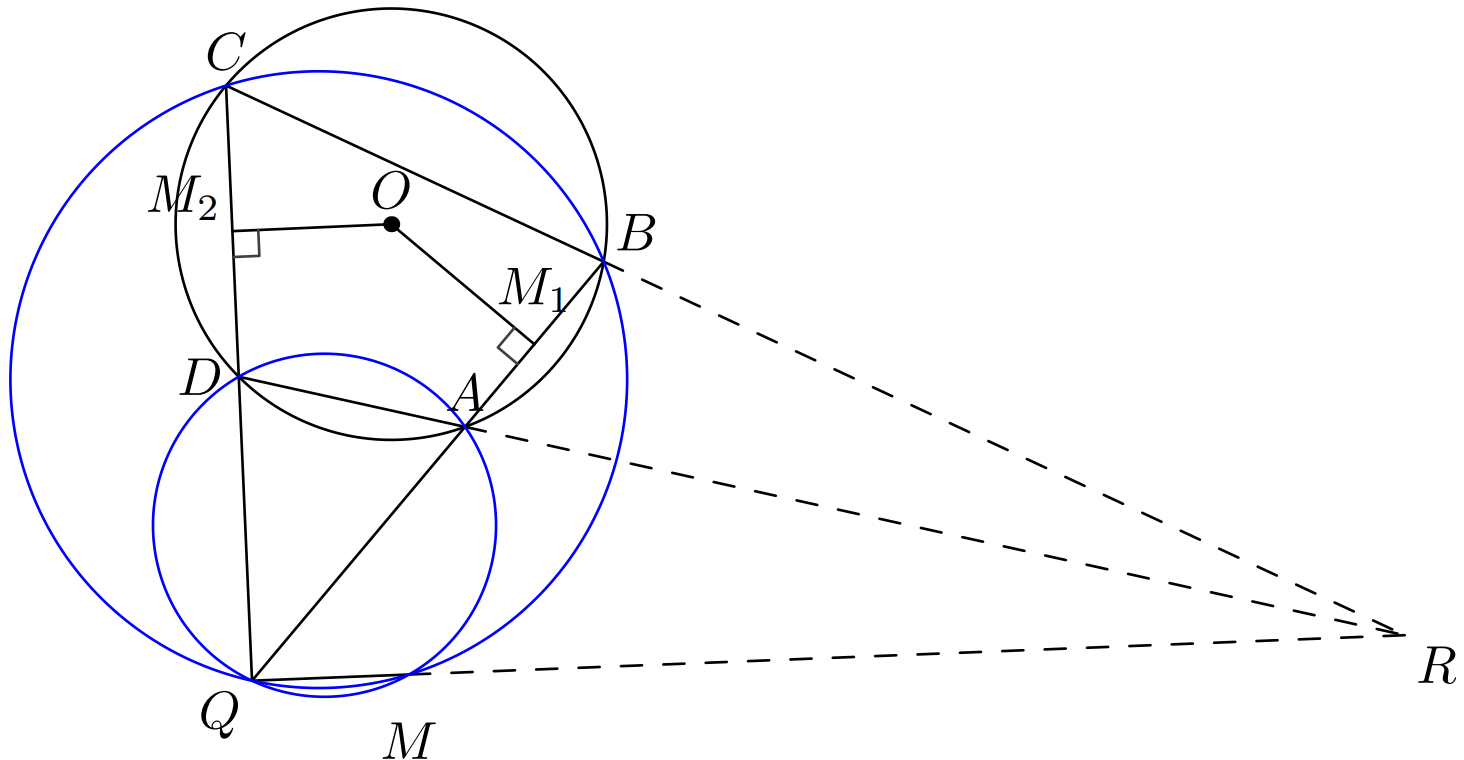
\includegraphics[scale=0.3]{p4.3}
	\caption{Diagrama para prueba del Hecho 8}
\end{figure}

Prueba. Utilicemos $\Tau$ para denotar la semejanza espiral centrada en $M$ que env\'ia a $A$ a $D$ y a $B$ a $C$ (Hecho 7). Sean $M_1$ y $M_2$ loes puntos medios de $AB$ y $DC$ respectivamente. Luego $\Tau$ debe env\'iar a $M_1$ a $M_2$. As\'i que $M$ es el centro de la \'unica semejanza espiral que env\'ia a $A$ a $M_1$ y $D$ a $M_2$ (Hecho 6), y por lo tanto $M, M_1, M2, Q$ son conc\'iclicos (Hecho 5).
Como $M_1$ y $M_2$ son los puntos medios de las cuerdas $AB$ y $DC$, tenemos $\angle OM_2Q = \angle OM_1Q$, y por lo tanto $O, M_1, M_2, Q$ son conc\'iclicos y $OQ$ es el diametro del c\'irculo en com\'un. Luego $O, M, M_1, M_2, Q $ est\'an en el c\'irculo con diametro $OQ$. En particular, $\angle OMQ = 90^{\circ}$, como quer\'iamos. \hfill $\square$
\end{document}
